\documentclass{iagtese} 		% declaração da classe iagtese com
						% padrões de formatação.
						%	
%\documentclass{iagtese_en}	% declaração da classe iagtese em
						% ingles. Para escrever a tese em 
						% ingles, descomente esta linha e 
						% comente a linha anterior.
						%				%	
%\hypercolor				% links coloridos para a versao
						% on line da tese. Para usar esta
						% opcao descomente esta linha.
						% 	
\begin{document}			% início do documento
						% 				
\institution{Universidade de São Paulo \\ Instituto de Astronomia, Geofísica e Ciências Atmosféricas \\ Departamento de Astronomia}

\title{Título do trabalho}

\translator{{Tese/Dissertação apresentada ao Departamento de Astronomia do Instituto de Astronomia, Geofísica e Ciências Atmosféricas da Universidade de São Paulo como requisito parcial para a obtenção do título de Mestre/{}Doutor em Ciências.\\ \\
Área de Concentração: Astronomia\\
Orientador(a): Prof.($^{\rm a}$) Dr.($^{\rm a}$) Orientador(a)}}

\author{Autor}

\date{São Paulo \ano}			% arquivo para inserir a capa
						%
\pagestyle{empty}			% padrão de formatação para parte
						% inicial do texto
						%
\maketitle					% 
						%
\Dedicatoria				%
\hfill
\vfill
\hfill{\it{sua dedicatoria aqui!}}
\vspace{2cm}		%
						% componentes iniciais do trabalho
\Agradecimentos			%
\addtotextpreliminarycontent{\lang{Acknowledgement}{Agradecimentos}}

\begin{agradecimentos}

\lang
{
    Greetings.
}
{
    Os agradecimentos principais são direcionados à Gerald Weber, Miguel Frasson,
    Leslie H. Watter, Bruno Parente Lima, Flávio de Vasconcellos Corrêa, Otavio Real
    Salvador, Renato Machnievscz\footnote{Os nomes dos integrantes do primeiro
    projeto abn\TeX\ foram extraídos de
    \url{http://codigolivre.org.br/projects/abntex/}} e todos aqueles que
    contribuíram para que a produção de trabalhos acadêmicos conforme
    as normas ABNT com \LaTeX{} fosse possível.

    Agradecimentos especiais são direcionados ao Centro de Pesquisa em Arquitetura
    da Informação\footnote{\url{http://www.cpai.unb.br/}} da Universidade de
    Brasília (CPAI), ao grupo de usuários
    \emph{latex-br}\footnote{\url{http://groups.google.com/group/latex-br}} e aos
    novos voluntários do grupo
    \emph{\abnTeX{}}\footnote{\url{http://groups.google.com/group/abntex2} e
    \url{http://abntex2.googlecode.com/}}~que contribuíram e que ainda
    contribuirão para a evolução do \abnTeX{}.
}

\end{agradecimentos}


%Mesmo padrão da seção primária, porém sem indicativo numérico. Assim como: Dedicatória, Resumo, Abstract, Sumário, Listas, Referências, Apêndices e Anexos.
%
%
%Corpo do texto, fonte 10,5, justificado, recuo especial da primeira linha de 1 cm, espaçamento simples.
%
	% caso não queira adicionar algum
						% deles, simplesmente remova as
						% linhas correspondentes.
						%
\Epigrafe					%  
% ---
% Epígrafe
% ---
\aspas{As invenções são, sobretudo, \\
o resultado de um trabalho de teimoso.}\\
		(Santos Dumont)
% ---		%
						%
\Resumo					%
Resumo		%
						%
\Abstract					%
Abstract		%
						%
\listoffigures 				% lista de figuras (opcional)
\listoftables 				% lista de tabelas (opcional)
\tableofcontents 			% sumário
						%
\cleardoublepage			%
\pagestyle{fancy}			% formatação para corpo do texto
						%
% Comando simples para exibir comandos Latex no texto
\newcommand{\comando}[1]{\textbf{$\backslash$#1}}

Este documento explica brevemente como trabalhar com a classe \LaTeX~\textit{icmc} para confeccionar trabalhos acadêmicos seguindo as normas da \sigla{ABNT}{Associação Brasileira de Normas Técnicas} e as \aspas{\textit{Diretrizes para apresentação de dissertações e teses da USP: documento eletrônico e impresso. Parte I (ABNT)}}, publicado pelo \sigla{SIBi}{Sistema Integrado de Bibliotecas} USP. O presente manual também atende as exigências prevista no regimento do Programa de Pós-graduação em \sigla{CCMC}{Ciências da Computação e Matemática Computacional} do \sigla{ICMC}{Instituto de Ciências Matemáticas e de Computação} da \sigla{USP}{Universidade de São Paulo}.


A classe \textit{icmc} foi construída com base na última versão da classe \textit{abntex2} e do pacote \textit{abntex2cite}. Portanto, este documento exemplifica a elaboração de trabalho
acadêmico (tese, dissertação e outros do gênero) produzido conforme a ABNT NBR
14724:2011 \textit{Informação e documentação - Trabalhos acadêmicos - Apresentação}.

Assim, é altamente recomendável que seja consultada a documentação do \textit{abntex2}\footnote{http://abntex.net.br}. A classe \textit{abntex2} foi desenvolvida para facilitar a escrita de documentos seguindo as normas da ABNT no ambiente \LaTeX\;\cite{frasson:2005:classe_abnt}.

Todo o trabalho de pesquisa e ajustes da presente classe \LaTeX~\emph{icmc} foram feitos pelo aluno mestrado do Programa de Pós-graduação em Ciência da Computação e Matemática Computacional, Humberto Lidio Antonelli, durante a confecção da sua monografia de qualificação.

O requisito básico para utilização da classe \textit{icmc} é criar um documento desta classe com o comando
\comando{documentclass[@parameters]\{icmc\}} e ter, no diretório de trabalho, o arquivo \emph{icmc.cls} presente. Entretanto, recomenda-se fortemente manter a estrutura de diretório inicial fornecida por este modelo. Além disso, para que o documento esteja em conformidade com as normas exigidas pelo programa de Pós-Graduação, o \textbf{projeto deve ser compilado utilizando \textit{XeLaTeX} ou \textit{LuaLaTeX}}. Esse processo de compilação é necessário para que as fontes externas utilizadas para gerar a capa sejam incluídas.

Os parâmetros possíveis utilizados pelo \comando{documentclass} são:
\begin{description}
\item[qualificacao] Exclusivamente para monografias de qualificação em geral;
\item[mestrado / doutorado] Identifica o curso ao qual o aluno pertence, sendo utilizado apenas uma das duas opcões disponíveis. O valor padrão é \textbf{doutorado};
\item[pre-defesa / pos-defesa] Identifica a situação do documento (exceto para qualificação), sedo necessário apenas uma das duas opções. O valor padrão é \textbf{pos-defesa};
\item[impressao] Gera exclusivamente uma versão para impressão do documento;
\item[french, spanish, english, brazil] Adiciona o idioma para correta hifenização correta no documento. Os idiomas bases para o modelo (português e inglês) não precisam ser declarados.
\end{description}
		%
\chapter{Base de dados}\label{database}

Base de dados. Citar figura \ref{identificador}.

\begin{figure}[!ht]
\begin{center}
\setcaptionmargin{1cm}
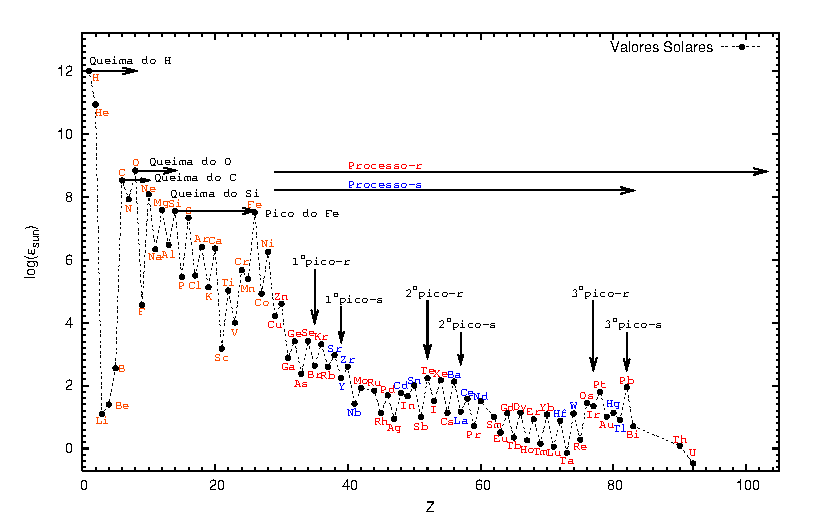
\includegraphics[width=1.0 \columnwidth,angle=0]{fig/solar_grevesse.eps}
\caption[Resumo da legenda da figura (aparece na lista de figuras)]{Legenda da figura.} 
\label{identificador}
\end{center}
\end{figure}


\begin{center}
\setcaptionmargin{1cm}
\scriptsize
\begin{longtable}{lcccc}
\caption[Resumo da legenda da tabela (aparece na lista de figuras)]{Exemplo de tabela feita com o longtable.}\\
\hline \hline \\[-2ex]
\multicolumn{1}{c}{Coluna1} &
\multicolumn{1}{c}{Coluna2} &
\multicolumn{1}{c}{Coluna3} &
\multicolumn{1}{c}{Coluna4} &
\multicolumn{1}{c}{Coluna5} 

\\[0.5ex] \hline
\\[-1.8ex]

\endfirsthead

\multicolumn{5}{c}{\footnotesize{{\slshape{{\tablename} \thetable{}}} - Continuação}}\\[0.5ex]

\hline \hline\\[-2ex]

\multicolumn{1}{c}{Coluna1} &
\multicolumn{1}{c}{Coluna2} &
\multicolumn{1}{c}{Coluna3} &
\multicolumn{1}{c}{Coluna4} &
\multicolumn{1}{c}{Coluna5} 

\\[0.5ex] \hline
\\[-1.8ex]

\endhead

\multicolumn{3}{l}{{\footnotesize{Continua na próxima página\ldots}}}\\
\endfoot
\hline

\endlastfoot

1 & 2 & 3 & 4 & 5 \\
6 & 7 & 8 & 9 & 10\\

\label{tabela_com_longtable}
\end{longtable}
\end{center}    	% inserir os capítulos do seu
\chapter{Análise}


Análise		% trabalho.
\chapter{Conclusões}\label{conc}

Conclusões do trabalho e/{}ou perspectivas		% 
       						%
						%
%\begin{thebibliography}{99}	% referências bibliográficas (dê
%\bibitem{Quireza et al. 2007}{quireza}Quireza C., Rocha-Pinto H. J., Maciel W. J., 2007, A\&A, 475, 217

\bibitem[Aoki et al.(2001)]{2001ApJ...561..346A} Aoki, W., Ryan, S. G., Norris, J. E., Beers, T. C., Ando, H., Iwamoto, N., Kajino, T., Mathews, G. J., \& Fujimoto, M. Y. 2001, ApJ 561, 346

\bibitem[Aoki et al.(2002)]{2002ApJ...580.1149A} Aoki, W., Ryan, S. G., Norris, J. E., Beers, T. C., Ando, H., \& Tsangarides, S. 2002, ApJ 580, 1149 

\bibitem[Wasserburg et al. (1994)]{1994ApJ...424..412W} Wasserburg, G. J., Busso, M., Gallino, R., \& Raiteri, C. M. 1994, ApJ 424, 412 	% preferência ao bibTeX).
%\end{thebibliography}		% caso não use o bibTeX, remova os
						% comentarios das três linhas
						% e comente a linha \bibliography
						%
\bibliography{tex/bibliografia}	% bibliografia utilizando bibTeX,
						% referente ao arquivo
						% bibliografia.bib na pasta tex/
						%
\begin{apendice}			% inicio do ambiente apendice
\chapter{título do apêndice 01}\label{ap01}

\section{subtítulo 01}\label{subap01}

\chapter{título do apêndice 02}\label{ap02}		% texto referente ao apendice
\end{apendice}				% fim do ambiente apendice. caso
						% nao utilize apendice, remova as
						% 3 linhas de comando.
						%
\end{document}				% fim do arquivo